% Chapter 1

\chapter{Adversarial Networks Training} % Main chapter title
\label{Chapter5} % For referencing the chapter elsewhere, use \ref{Chapter1} 

\begin{figure}
\centering
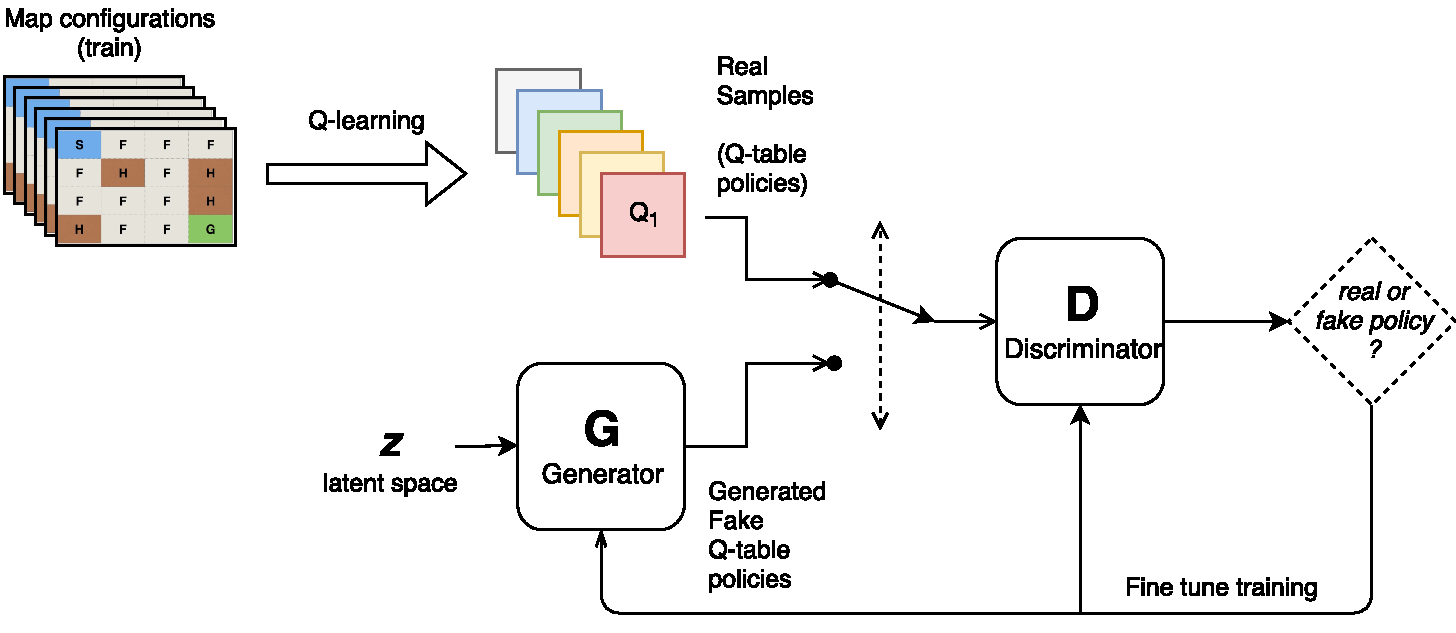
\includegraphics[width=15cm]{Figures/Q-GAN}
\caption{Our Generative Adversarial Network architecture}
\label{fig:Generator}
\end{figure}

%----------------------------------------------------------------------------------------


% TODO: Here I'll describe my architecture for both networks, show some interesting snippets of the PyTorch code to run the training on GPU. I'll motivate design decisions for the architecture of both generator and discriminator (why the number of hidden layers, and the number of nodes).


\section{Generator}
\begin{figure}
\centering
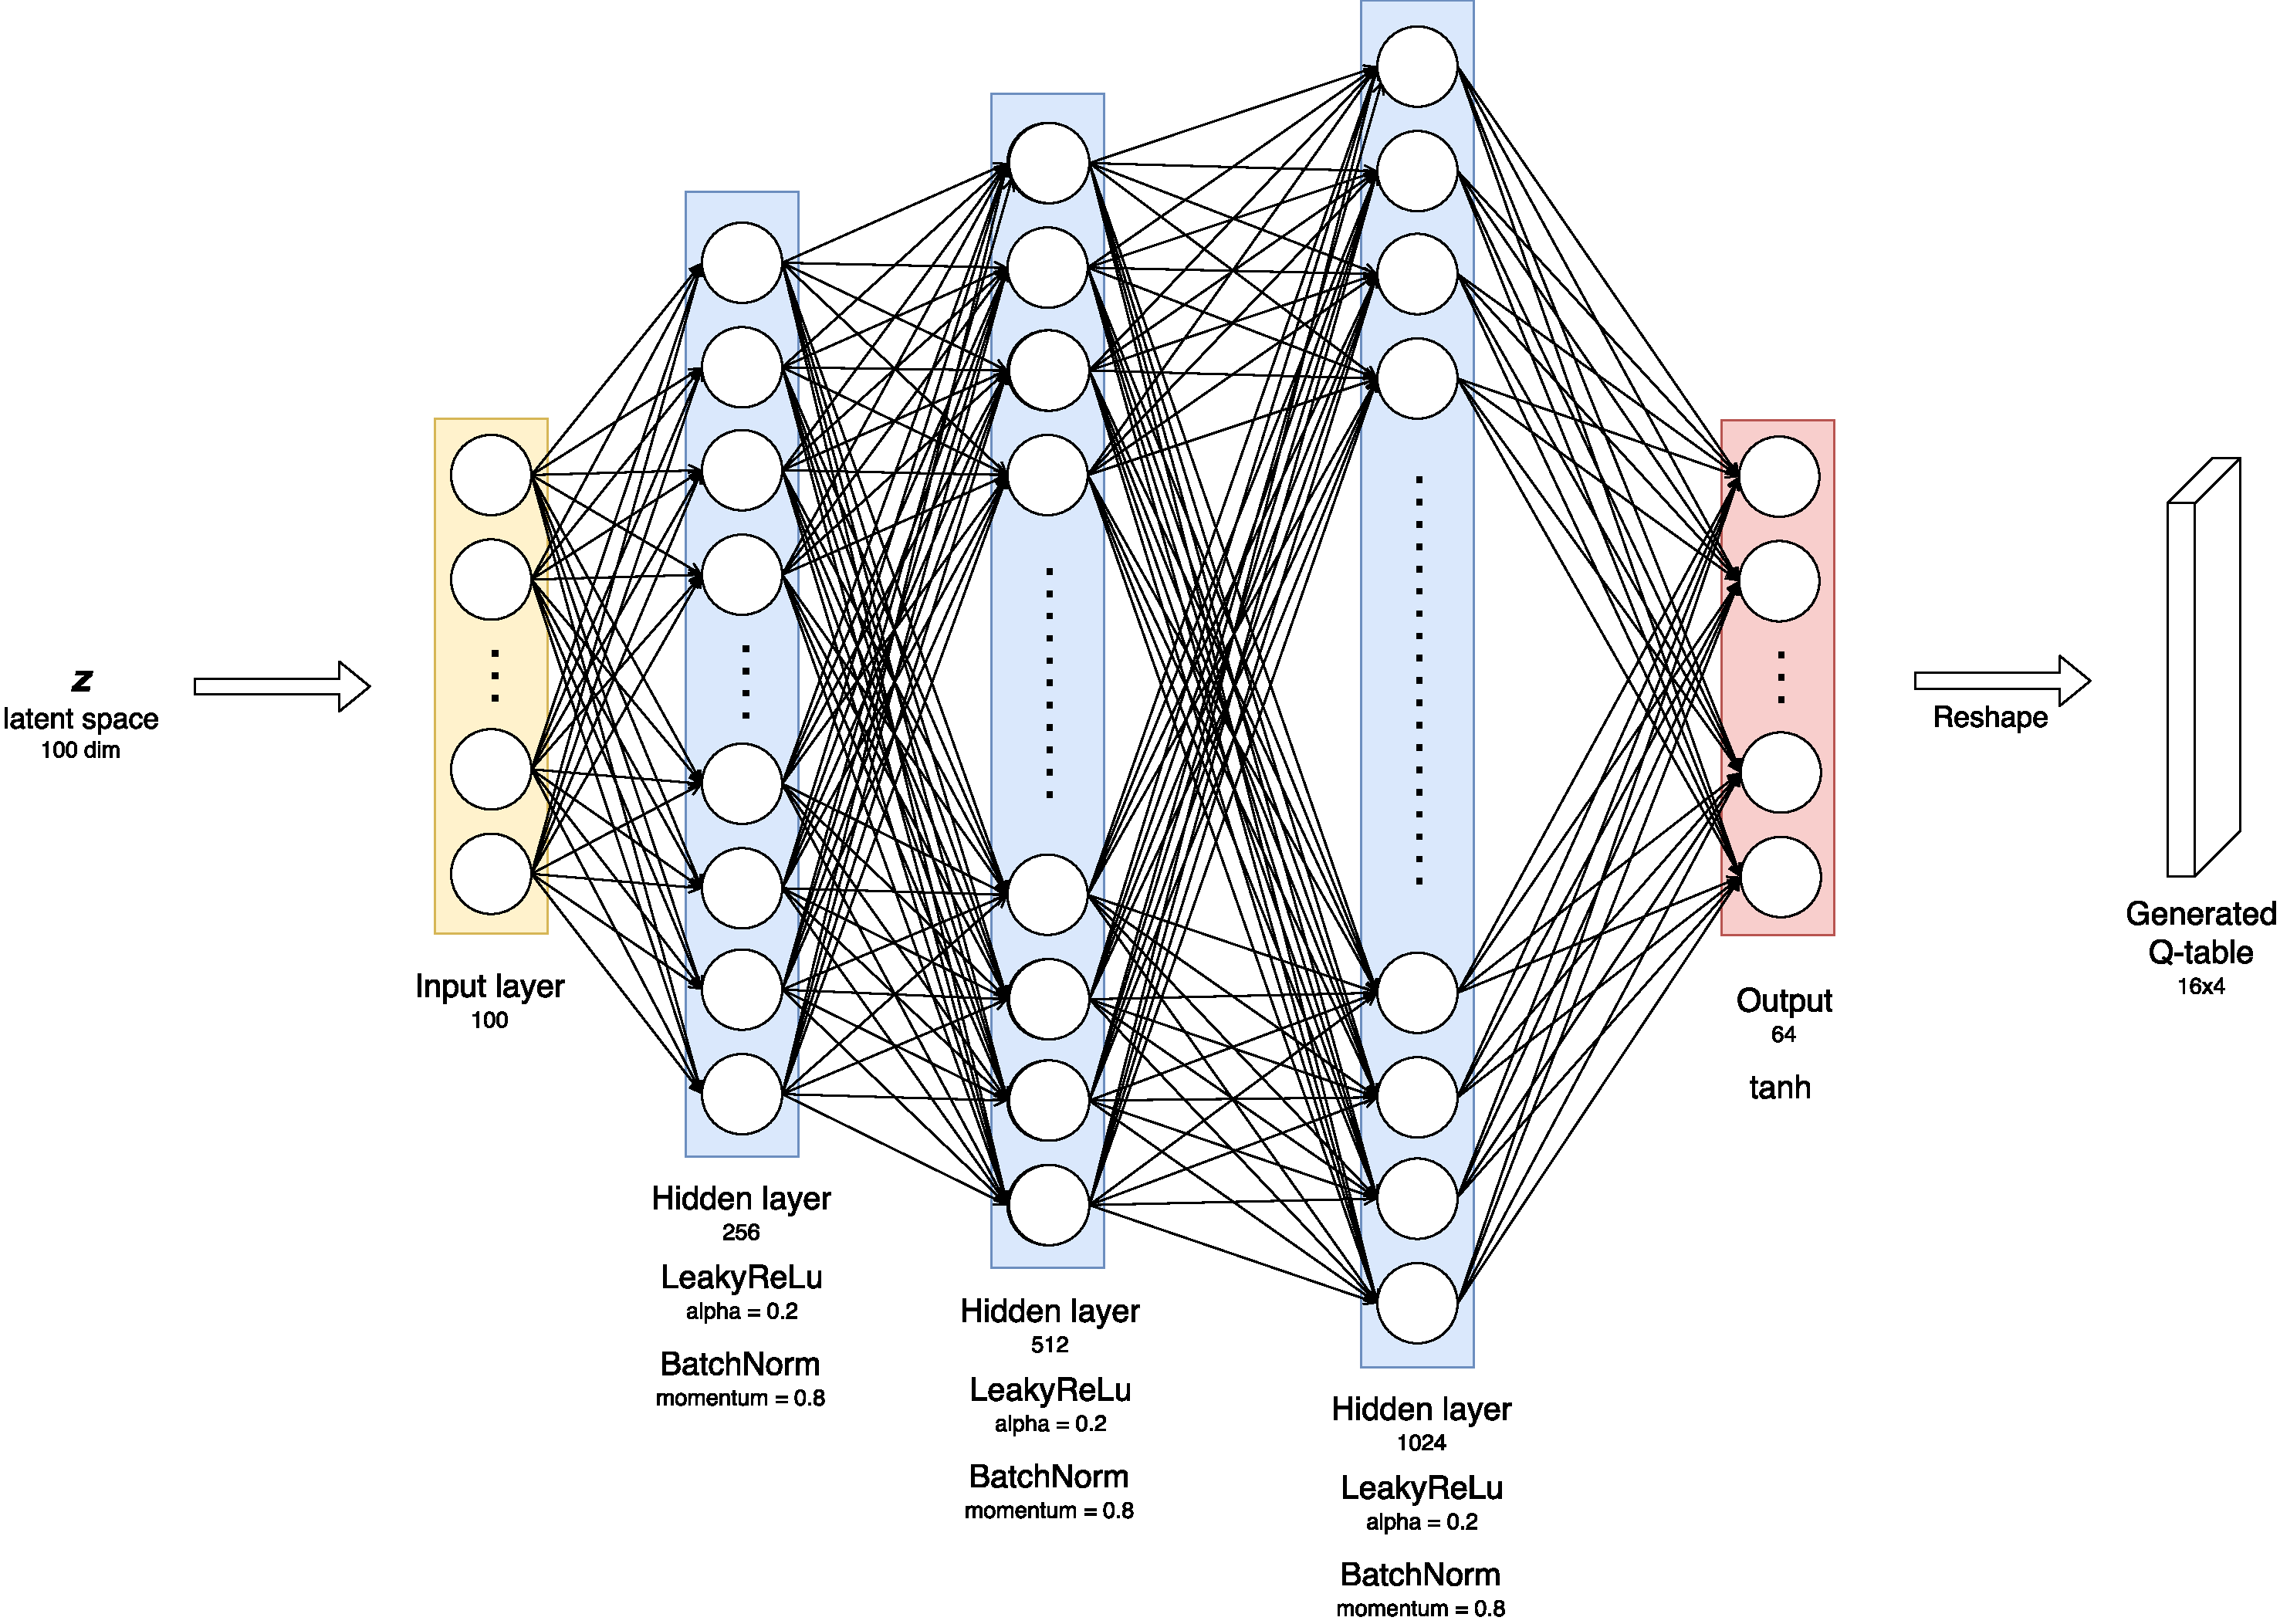
\includegraphics[width=15cm]{Figures/Generator}
\caption{Architecture of the Generator network}
\label{fig:Generator}
\end{figure}

\section{Discriminator}
\begin{figure}
\centering
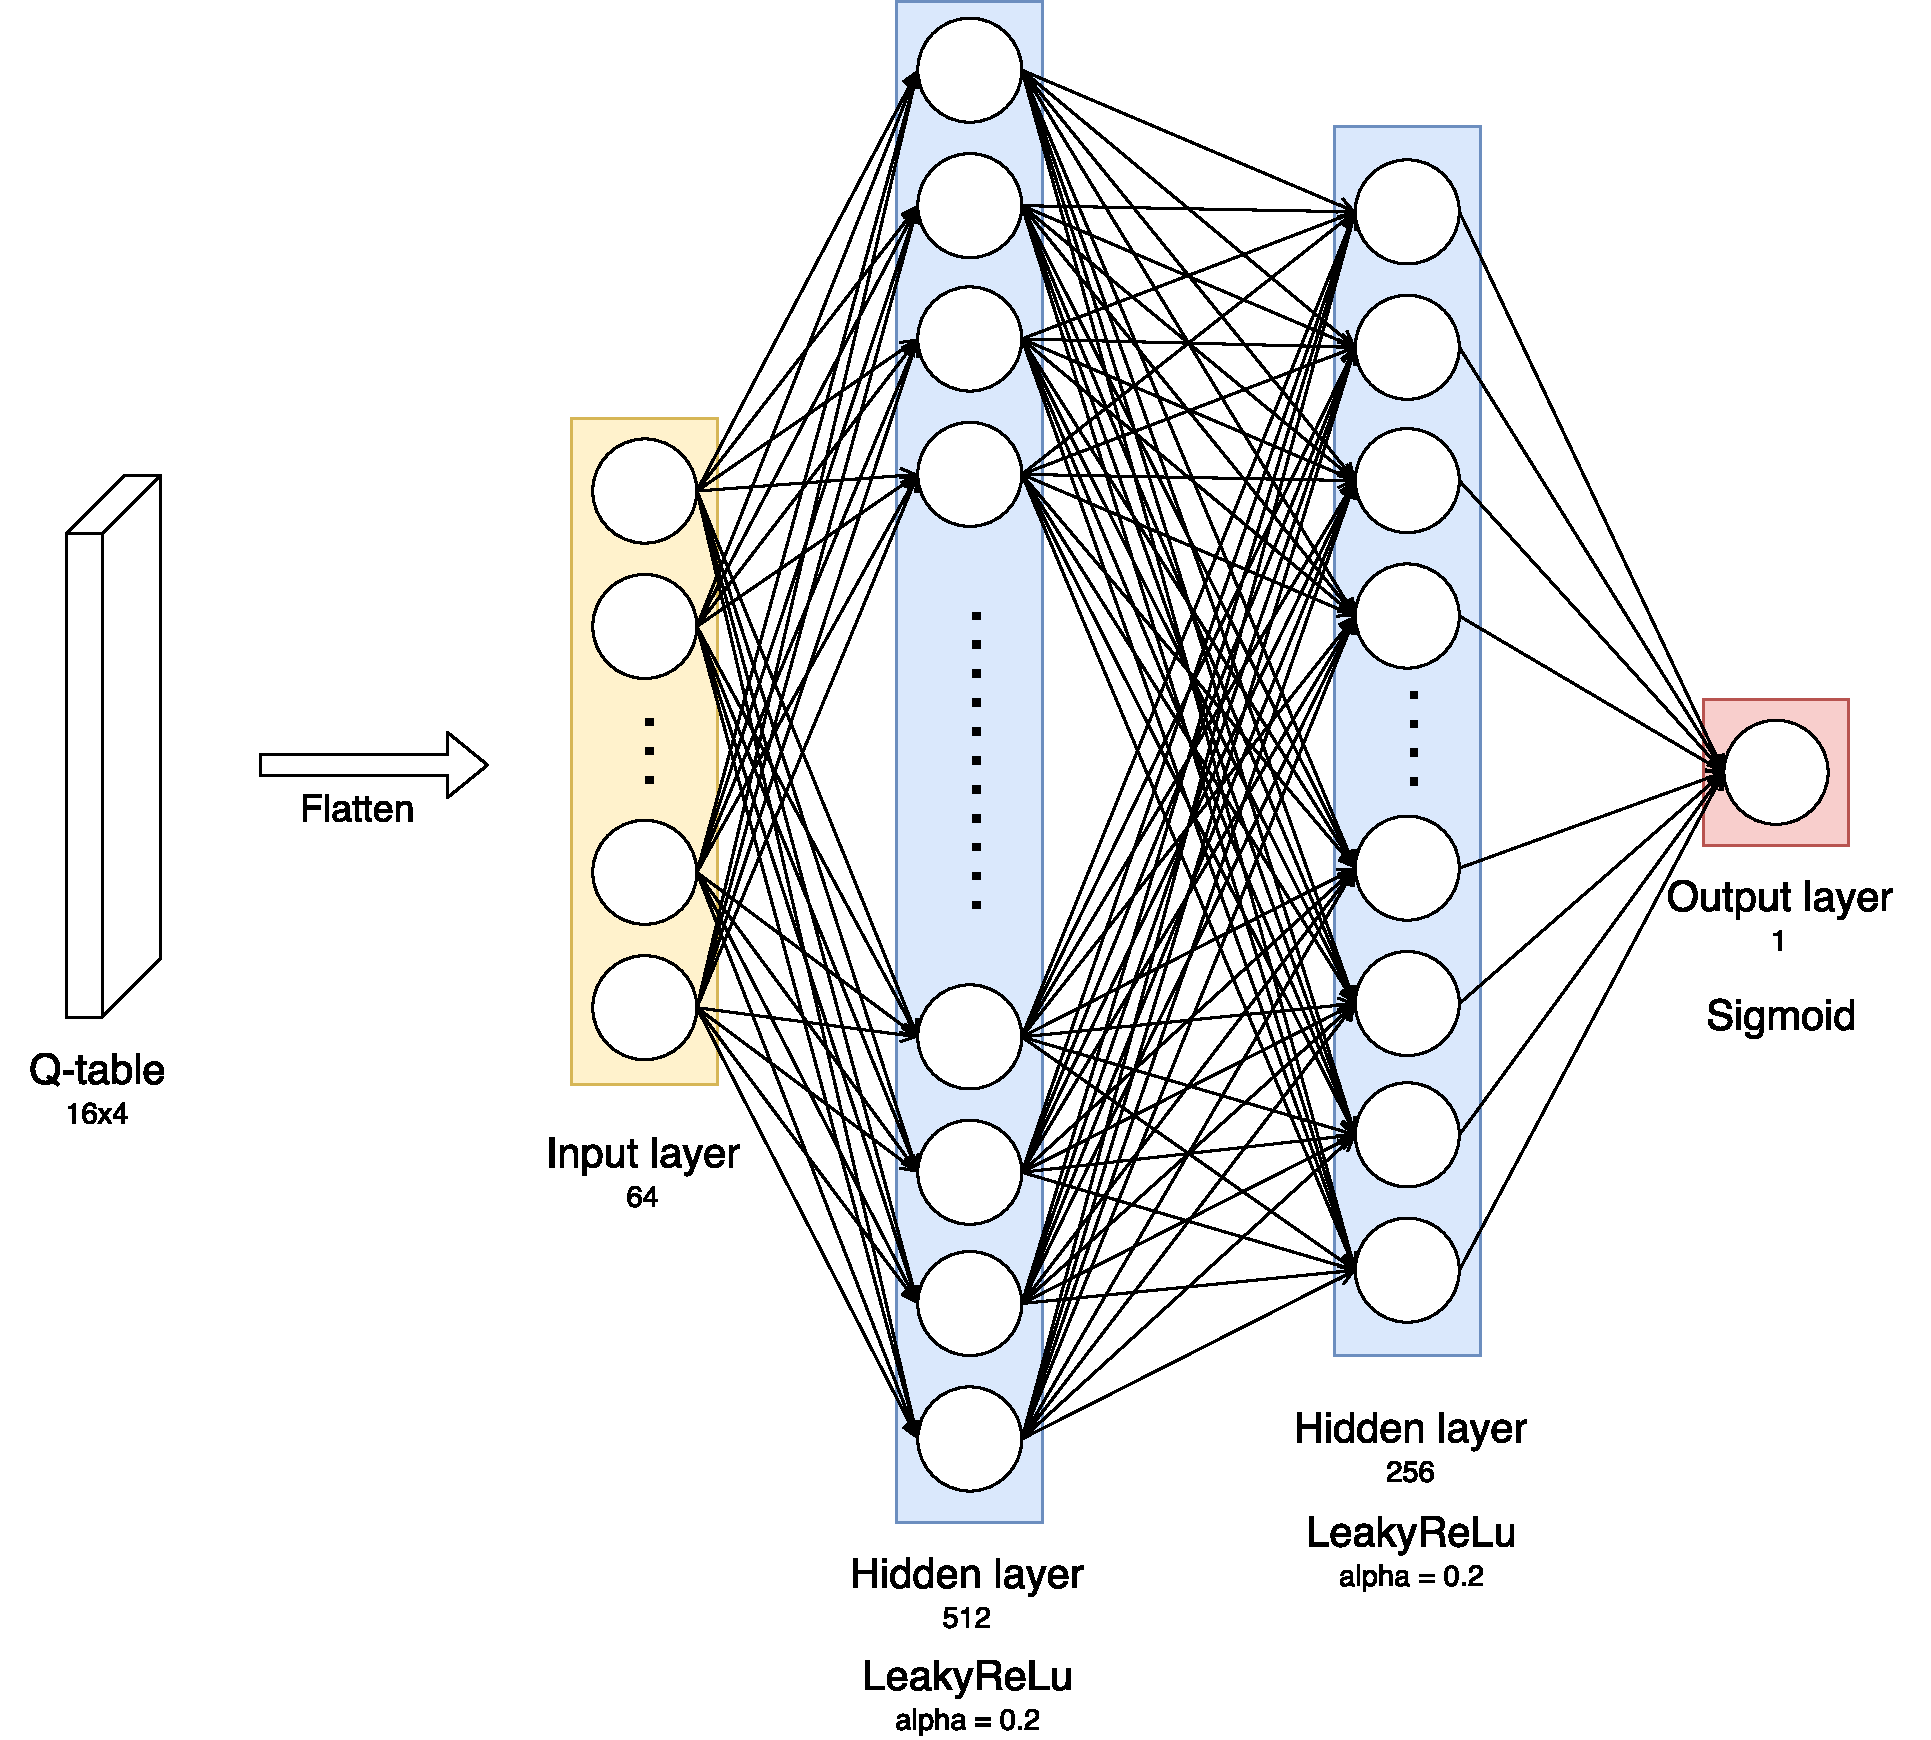
\includegraphics[width=10cm]{Figures/Discriminator}
\caption{Architecture of the Discriminator network}
\label{fig:Generator}
\end{figure}